\chapter{Analysis}\label{ch:analysis}

Sonar Workbench includes built-in functions to assist with analysis.  Versions 1.0-3.0 concentrated on array building, conventional beam pattern synthesis, and beam pattern analysis.  Planned upgrades include support for adaptive beamforming, element and array radiation impedance, and array gain in anisotropic noise.

\section{Plotting arrays}

The function \texttt{PlotArray.m} creates a 3D plot of an array. Usage instructions are shown in Listing~\ref{lst:PlotArray}. The user must pass the array structure as the first parameter to \texttt{PlotArray.m}. This will produce a physical plot of the array, as shown in \figname~\ref{fig:SampleArray}. There are three optional inputs to \texttt{PlotArray.m}. The user can enter empty brackets \texttt{[]} for any optional parameters that are not needed. If the user inputs a beam structure in the second parameter, the elements will be filled with a solid color whose opacity is proportional to the amplitude weights, as shown in \figname~\ref{fig:SampleBeam}. To plot the array in an existing figure axis, pass a handle to that axis as the third parameter, \texttt{hax}. The Matlab function \texttt{gca} can be used to specify the current axis. The fourth parameter lets the user plot the array scaled to dimensions of 1 unit = 1 meter. This is helpful if the array is to be overlaid on a user-generated plot of its host platform. The fifth and final parameter lets the user specify the color to use for each element. This input is a 3-element normalized vector containing red, green, and blue color components.

\newpage
\lstinputlisting[firstline=2,lastline=35,caption={\texttt{PlotArray.m}},label={lst:PlotArray}]{../../mdl/PlotArray.m}
 
\section{Calculating beam patterns}

\texttt{BeamPattern.m} calculates the beam pattern for wavelength $\lambda$, elevation angles $\theta$, and azimuthal angles $\psi$ as
\begin{equation}
BP(\lambda,\theta,\psi) = \sum_{i=1}^{N_e} w_i(\lambda,\theta_0,\psi_0)E_i(\lambda,\theta,\psi)e^{j2\pi\left(\frac{\cos\theta\cos\psi}{\lambda}x_i + \frac{\cos\theta\sin\psi}{\lambda}y_i + \frac{\sin\theta}{\lambda}z_i\right)},
\end{equation}
where, for the $i^{th}$ element in the array, $w_i(\lambda,\theta_0,\psi_0)$ is the complex weight, $E_i(\lambda,\theta,\psi)$ is the element pattern, rotated according to the element orientation ($\gamma_i$,$\theta_i$,$\psi_i$), and ($x_i$,$y_i$,$z_i$) are the element coordinates. This computation is performed in the body frame. To calculate the beam pattern in the array frame, set the array position and orientation to [0;0;0].

The beam pattern is returned in complex linear units. This retains the amplitude and phase information from the beam. By default, the amplitude is normalized by dividing the output by the sum of the beam weight amplitudes,
\begin{equation}
BP_{norm}(\lambda,\theta,\psi) = \frac{BP(\lambda,\theta,\psi)}{\sum_{i=1}^{N_e}|w_i(\lambda,\theta_0,\psi_0)|}.
\end{equation}
For an unsteered beam, this produces an output with amplitude 1 along the maximum response axis. Steering beams off axis can result in a peak beam amplitude less than 1. The user can also choose to normalize the beam pattern relative to the peak calculated value or skip the normalization step altogether.

Usage instructions for \texttt{BeamPattern.m} are shown in Listing~\ref{lst:BeamPattern}. The first two input parameters are the array and beam structures. The third parameter is the wavelength, $\lambda$, in meters. This must be a scalar. 

The final required parameters are the elevation and azimuthal angles over which the beam pattern is to be calculated, in degrees. These parameters can be scalars, vectors, or matrices, but they must have compatible dimensions. If both are scalars, the output, \texttt{BP}, will be a scalar. If both are column vectors of the same length or matrices with identical dimensions, \texttt{BeamPattern.m} treats them as coordinate pairs at which to evaluate the beam pattern. If \texttt{theta} is a column vector and \texttt{psi} is a row vector, \texttt{BeamPattern.m} uses the Matlab function \texttt{ndgrid} to calculate a matrix \texttt{BP}, with rows corresponding to constant $\theta$ and columns corresponding to constant $\psi$. The user can generate their own matrix inputs using \texttt{[Theta,Psi] = ndgrid(theta,psi);} for vectors \texttt{theta} and \texttt{psi}.

After the required parameters, a single optional parameter, \texttt{NormMethod},  selects the method to use for beam pattern normalization, as shown in Table~\ref{tab:BeamPatternNormMethod}.

\begin{table}[!ht]
	\begin{center}
		\caption{\texttt{NormMethod} options for \texttt{BeamPattern.m}}
		\label{tab:BeamPatternNormMethod}
		\begin{tabular}{c|l} 
			\texttt{NormMethod} & \textbf{Description} \\
			\hline
			0 & No normalization\\
			1 & Normalize by beam pattern weights \\
			2 & Normalize by peak calculated beam pattern value\\
		\end{tabular}
	\end{center}
\end{table}

\clearpage

\lstinputlisting[firstline=2,lastline=41,caption={\texttt{BeamPattern.m}},label={lst:BeamPattern}]{../../mdl/BeamPattern.m}

\section{Extracting 2D slices from 3D beam patterns}

The function \texttt{ExtractBeamSlice.m} extracts a 2D slice from a 3D beam pattern by extracting all values that lie in a plane with user-specified orientation. Common usage includes extracting horizontal and vertical beam patterns for generating 2D plots, but the plane can also be rotated to different angles between horizontal and vertical. 

Listing~\ref{lst:ExtractBeamSlice} shows usage instructions for \texttt{ExtractBeamSlice.m}. All input parameters are required. The first two are the vertical and horizontal angles over which the beam pattern is evaluated, and the third input is the 3D beam pattern. The third input is a three-element orientation vector containing the roll, pitch, and yaw angles (in degrees) that rotate the default horizontal plane to the desired orientation. The first element of \texttt{Ori} is the roll parameter. Set this value to 0 for a horizontal slice and set it to -90 for a vertical slice. Other rotational angles can be useful, e.g. 60 for measuring the beam pattern of a haxagonal piston element along one of its axes of symmetry. The final two elements of \texttt{Ori} are the elevation and azimuth coordinates of the 2D slice's angular origin. Setting these elements to $\theta_0$ and $\psi_0$ places the center of the extracted 2D slice at a steered beam's maximum response axis. \texttt{ExtractBeamSlice.m} returns a vector of complex beam pattern values, \texttt{BPslice},  and a vector of angles, \texttt{phi}.

\lstinputlisting[firstline=2,lastline=21,caption={\texttt{ExtractBeamSlice.m}},label={lst:ExtractBeamSlice}]{../../mdl/ExtractBeamSlice.m}

Since \texttt{ExtractBeamSlice.m} outputs values defined over an angular span with fixed 1$^\circ$ spacing, and it uses interpolation to estimate values from coordinates that do not map directly to coordinates in the 3D beam pattern, it is best suited for visualization when a 3D beam pattern has already been calculated. For more precise results, evaluate \texttt{BeamPattern.m} at the desired $\theta$ and $\psi$ corresponding to the plane of interest directly. 

\section{Plotting 2D beam patterns}

The function \texttt{Plot2DBP.m} plots the two dimensional beam pattern magnitude with decibel scaling. Listing~\ref{lst:Plot2DBP} shows usage instructions. The two required inputs are the angle vector, $\phi$ in degrees, and the beam pattern vector.

The first optional input, \texttt{PlotType} selects from two different rectangular plots and two different polar plots, as listed in Table~\ref{tab:Plot2DBPlotType}. The first two plot types are suitable for displaying horizontal beam pattern slices or slices cut through any plane, while the third and fourth plot types are suitable for vertical beam pattern slices, according to the coordinate conventions used by Sonar Workbench. \figurename~\ref{fig:Plot2DBPexamples} shows examples of each plot type for 2D horizontal and vertical slices through the rectangular planar array's 3D beam pattern.

\begin{table}[!ht]
	\begin{center}
		\caption{\texttt{PlotType} options for \texttt{Plot2DBP.m}}
		\label{tab:Plot2DBPlotType}
		\begin{tabular}{c|l} 
			\texttt{PlotType} & \textbf{Description} \\
			\hline
			1 & Rectangular plot, 0$^\circ$ up, $+\phi$ right \\
			2 & Polar plot, 0$^\circ$ up, $+\phi$ clockwise \\
			3 & Rectangular plot, 0$^\circ$ right, $+\phi$ up \\
			4 & Polar plot, 0$^\circ$ right, $+\phi$ counterclockwise \\
		\end{tabular}
	\end{center}
\end{table}

The second optional input, \texttt{dBScale}, is a two-element vector with the minimum and maximum magnitudes in dB. The default values are -40 and 0 dB. It is common to use 0 dB for the maximum value, since the beam pattern is normalized by default.

The third optional input is the axis handle, \texttt{hax}, in which to plot the beam. This input has the same functionality as it does in \texttt{PlotArray.m}, and it allows the beam to be plotted with the array on the same axis. Matlab function \texttt{gca} can be used to specify the current axis.

\texttt{Plot2DBP.m} returns a single optional output, which is a handle to the plotted data. This allows the user to change the plot's appearance, such as line color and weight or marker type and size.

\lstinputlisting[firstline=2,lastline=28,caption={\texttt{Plot2DBP.m}},label={lst:Plot2DBP}]{../../mdl/Plot2DBP.m}

\clearpage
\begin{sidewaysfigure}[!ht]
\begin{center}
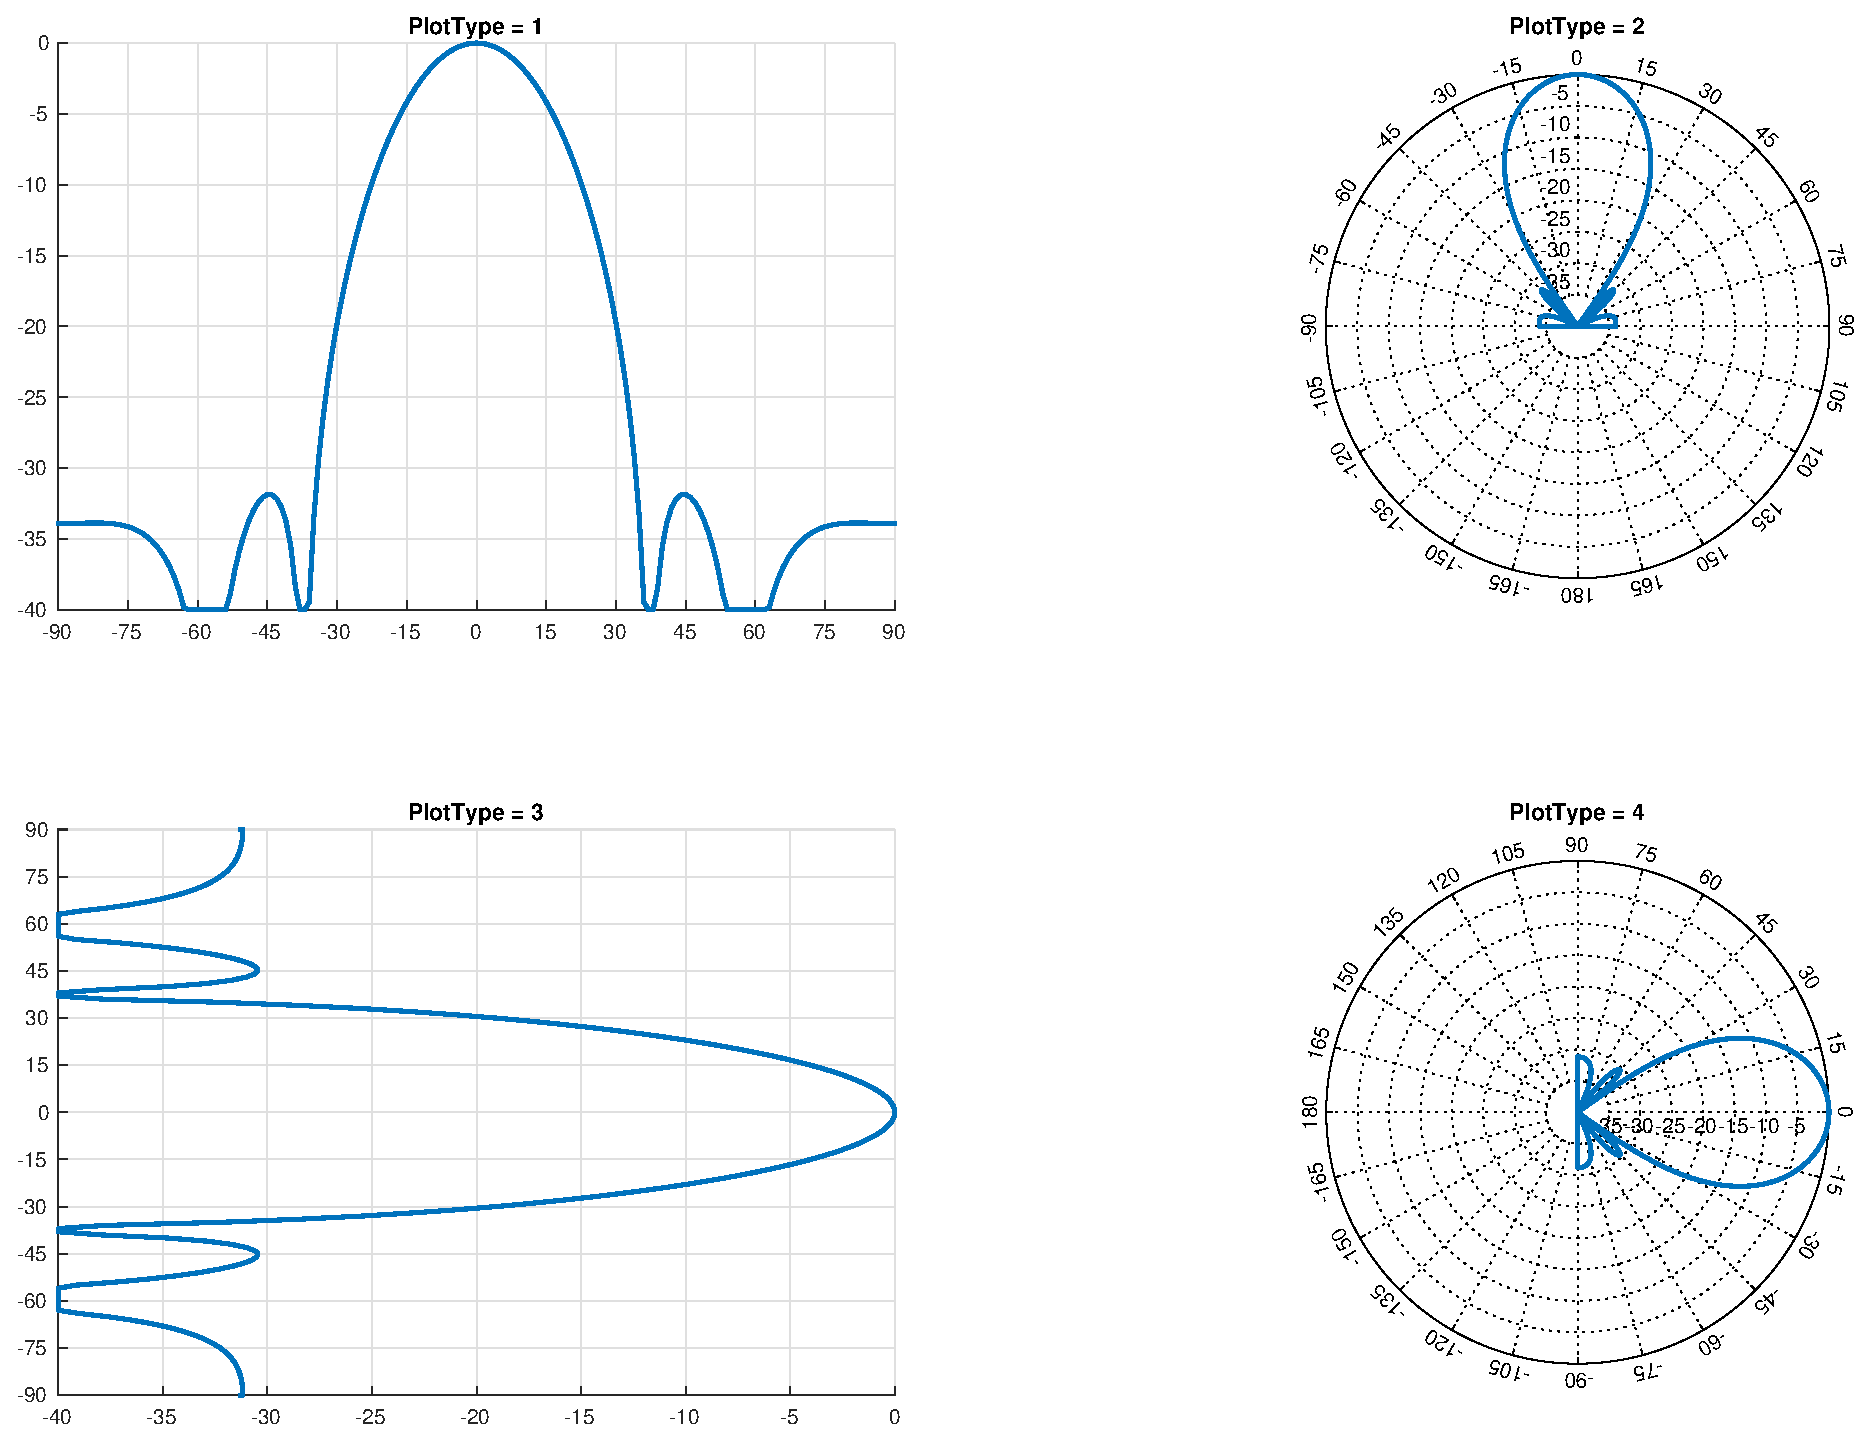
\includegraphics[width=7.75in]{Plot2DBPexamples}
\caption{\label{fig:Plot2DBPexamples}Example slices through rectangular planar array beam pattern}
\end{center}
\end{sidewaysfigure}

\clearpage
\section{Plotting 3D beam patterns}

The function \texttt{Plot3DBP.m} plots the three dimensional beam magnitude with decibel scaling. Usage instructions are shown in Listing~\ref{lst:Plot3DBP}. The three required inputs are elevation and azimuthal angle vectors, $\theta$ and $\psi$ in degrees, and the beam pattern matrix. 

The first optional input, \texttt{PlotType}, selects a plot with the beam pattern surface and color proportional to magnitude when its value is 1, and it selects a pot with the beam pattern color proportional to magnitude but drawn on a surface of constant radius when its value is 2. Examples of these two options are shown in the left and right panels of \figname~\ref{fig:SampleBeam} Those plots are for the example element, array, and beam defined in Listings~\ref{lst:SampleElement}, \ref{lst:SampleArray}, and \ref{lst:SampleBeam}.

The second optional input, \texttt{dBScale}, is a two-element vector with the minimum and maximum magnitudes in dB. The default values are -40 and 0 dB. It is common to use 0 dB for the maximum value, since the beam pattern is normalized by default.

The third optional input is the axis handle, \texttt{hax}, in which to plot the beam. This input has the same functionality as it does in \texttt{PlotArray.m}, and it allows the beam to be plotted with the array on the same axis. Matlab function \texttt{gca} can be used to specify the current axis.

The final optional inputs allow the beam to be offset according to the array position in the body frame. 

\lstinputlisting[firstline=2,lastline=26,caption={\texttt{Plot3DBP.m}},label={lst:Plot3DBP}]{../../mdl/Plot3DBP.m}

\clearpage
\begin{sidewaysfigure}[!ht]
\begin{center}
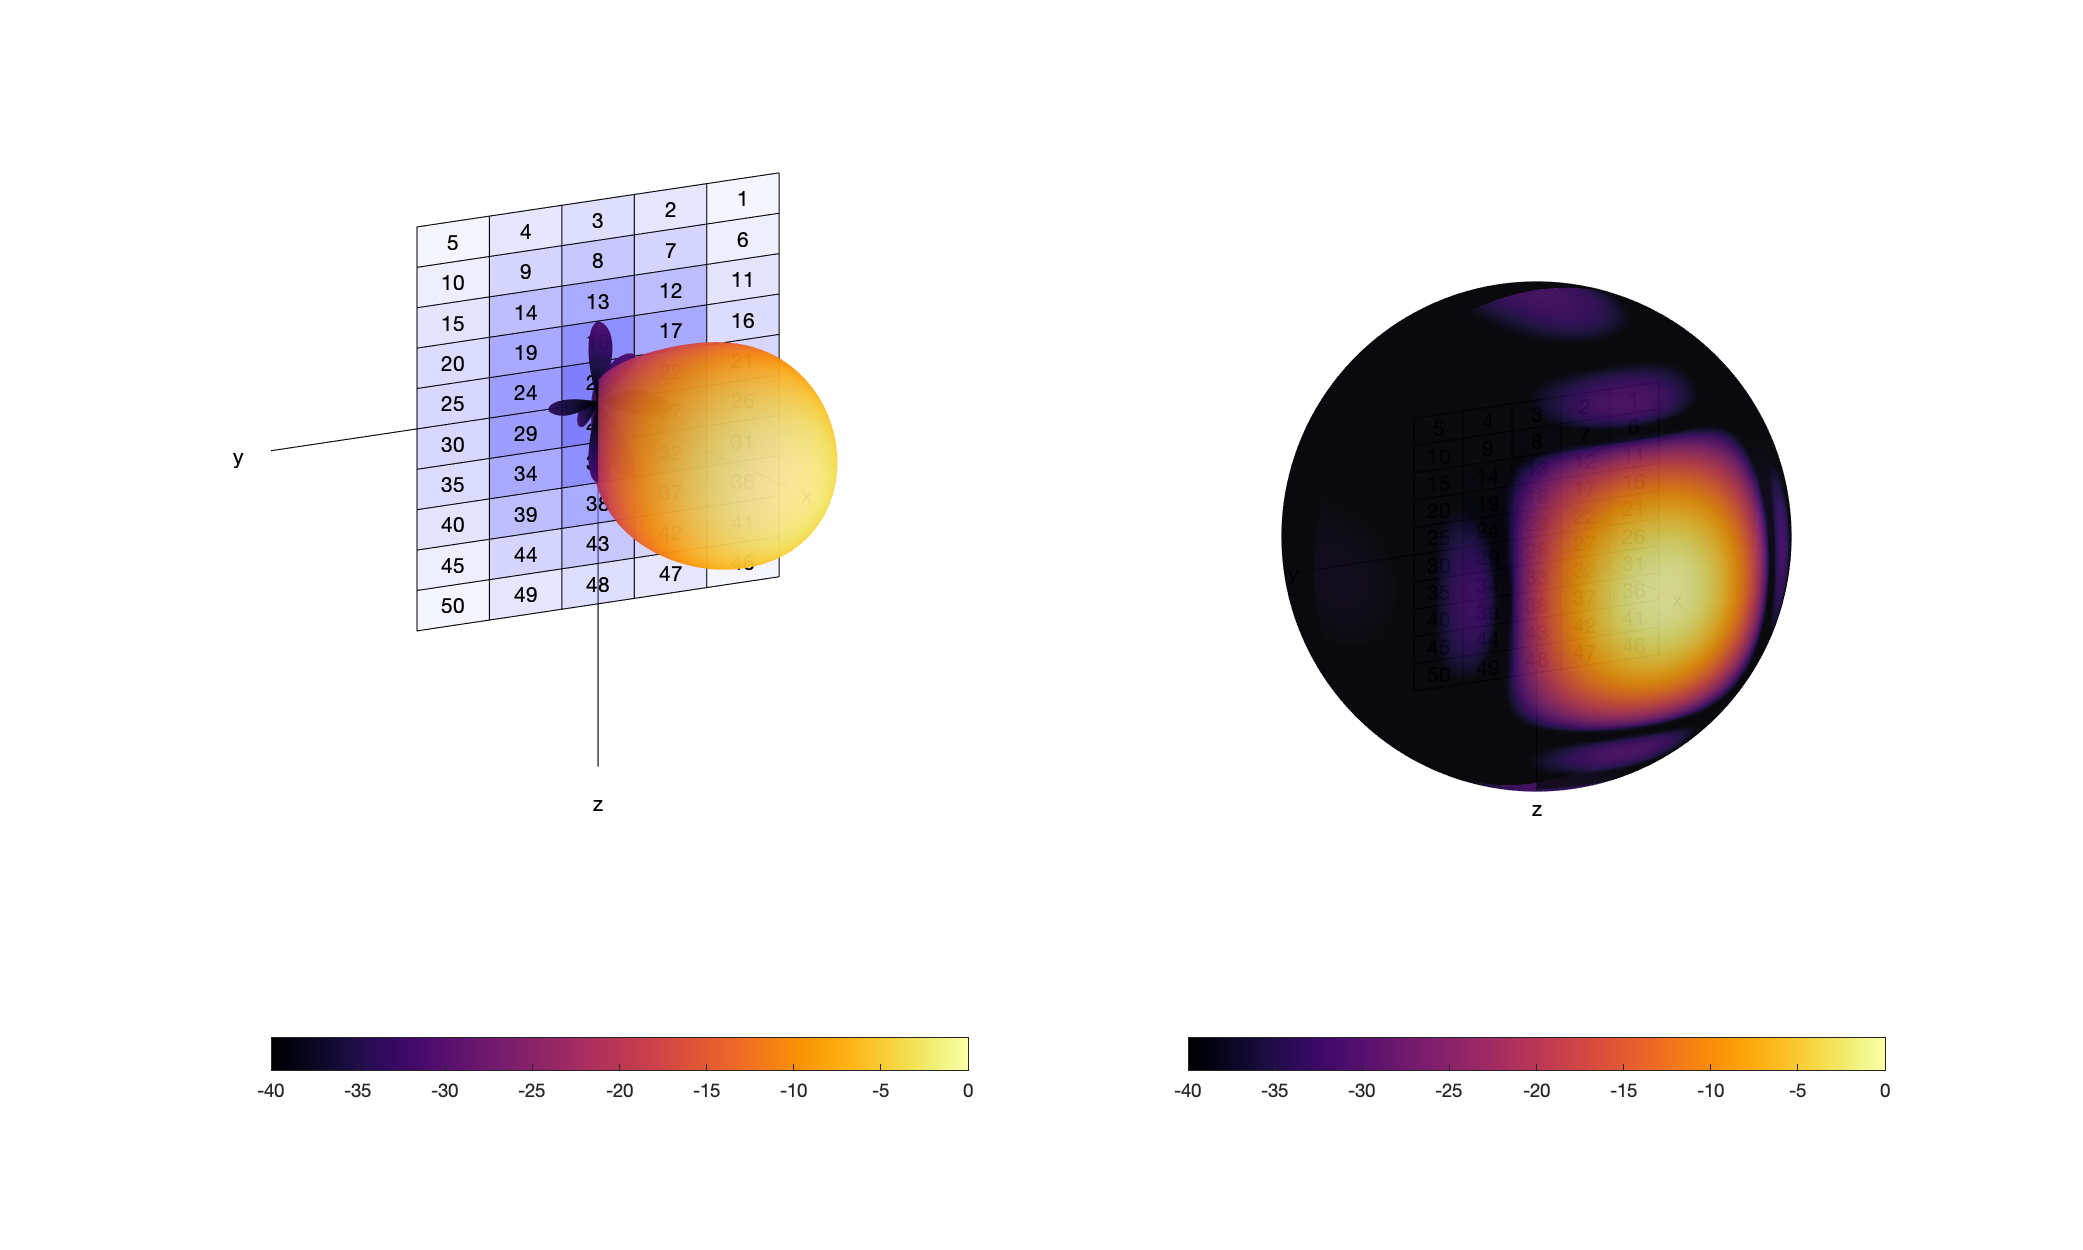
\includegraphics[width=7.75in]{SampleBeam}
\caption{\label{fig:SampleBeam}Example beam pattern for rectangular planar array}
\end{center}
\end{sidewaysfigure}

\clearpage
\section{Calculating beam width}

Beam width is the angular span over which the beam magnitude is within 3 dB of its peak value. Sonar Workbench contains two functions to calculate beam width: \texttt{BeamWidth.m} for 2D beams, which computes beam width in a single plane, and \texttt{BeamWidth3D.m} for 3D beams, which computes vertical and horizontal beam widths. Usage is shown in Listings~\ref{lst:BeamWidth} and \ref{lst:BeamWidth3D}.

\lstinputlisting[firstline=2,lastline=21,caption={\texttt{BeamWidth.m}},label={lst:BeamWidth}]{../../mdl/BeamWidth.m}

\lstinputlisting[firstline=2,lastline=26,caption={\texttt{BeamWidth3D.m}},label={lst:BeamWidth3D}]{../../mdl/BeamWidth3D.m}

There are two required parameters for \texttt{BeamWidth.m}. The first, \texttt{ang}, is a vector of angles in degrees over which the beam pattern slice is defined, and the second, \texttt{bp}, is the beam pattern at those angles, in linear units. The user can assist the function in locating the correct peak value to search around by specifying an approximate peak angle in the first optional parameter, \texttt{ang0}. The final optional parameter, \texttt{renorm}, instructs the function to re-normalize the beam pattern to have a peak magnitude of 0 dB before searching for the -3 dB angles. This can be useful for a steered beam whose peak magnitude is less than 0 dB. 

The output, \texttt{BW}, is the measured beam width in degrees. The function attempts to interpolate between input grid angles using spline interpolation of the beam magnitude in dB. The user can get a more precise measurement by using finer angle sampling. If \texttt{BeamWidth.m} can not calculate a valid beam width, it returns \texttt{NaN}.

\texttt{BeamWidth3D} has similar usage but with expanded support for an additional dimension. Its first three parameters are required, and correspond to angle vectors $\theta$ and $\psi$ in degrees and beam pattern matrix \texttt{BP} in linear units. The first two optional parameters, \texttt{theta0} and \texttt{psi0} serve the same purpose as \texttt{ang0} in \texttt{BeamWidth.m} for the elevation and azimuthal angles, respectively. The final optional parameter, \texttt{renorm}, is identical to that parameter in \texttt{BeamWidth.m}. There are two outputs, \texttt{BWV} and \texttt{BWH}, which are the vertical and horizontal beam widths in degrees, respectively. For the example beam in \figname~\ref{fig:SampleBeam}, the vertical and horizontal beam widths are calculated to be 26$^\circ$ and 25.6$^\circ$.

\section{Calculating directivity index}

Directivity Index (DI) is a measure of a beam's ability to filter spatially isotropic noise. It is the ratio of the noise level received by an omnidirectional sensor to the noise level received by the beam, expressed in dB. It is calculated from the Directivity (D) according to
\begin{equation}
DI(\lambda) = 10\log_{10}D(\lambda),\label{eq:DirectivityIndex}
\end{equation}
where
\begin{equation}
D(\lambda) = \frac{4\pi}{\int_0^{\pi}\int_0^{2\pi}|BP(\lambda,\theta,\psi)|^2d\psi{d\theta}}.\label{eq:Directivity}
\end{equation}

\texttt{CalculateDI.m} implements \eqnnames~(\ref{eq:DirectivityIndex}) and (\ref{eq:Directivity}) using numerical integration over a realized beam pattern. Usage is shown in Listing~\ref{lst:CalculateDI}.

There are three required parameters. The first two are angle vectors $\theta$ and $\psi$ in degrees, and the third is the beam pattern matrix \texttt{BP} in linear units. For best results, $\theta$ should span 180$^\circ$ vertically, and $\psi$ should span 360$^\circ$ horizontally. If instead, the beam pattern is defined as a subset of these angles, \texttt{CalculateDI.m} assumes the beam pattern value is exactly zero outside the defined region. There is a single output, \texttt{DI}, which is the directivity index in dB.

\lstinputlisting[firstline=2,lastline=18,caption={\texttt{CalculateDI.m}},label={lst:CalculateDI}]{../../mdl/CalculateDI.m}